% THIS IS AN EXAMPLE DOCUMENT FOR VLDB 2010
% based on ACM SIGPROC-SP.TEX VERSION 2.7
% Modified by  Gerald Weber <gerald@cs.auckland.ac.nz>


% This example *does* use the .bib file (from which the .bbl file
% is produced). REMEMBER HOWEVER: After having produced the .bbl file,
% and prior to final submission, you need to 'insert'  your .bbl file into
% your source .tex file so as to provide ONE 'self-contained' source file.

\documentclass[a4paper,12pt,oneside,titlepage]{book}
\renewcommand{\baselinestretch}{1.5}

%==============================================================
\usepackage[BoldFont, SlantFont, CJKchecksingle]{xeCJK}
\setCJKmainfont[Mapping=tex-text]{DFKai-SB}
\setCJKsansfont[Mapping=tex-text]{DFKai-SB}
\setCJKmonofont[Mapping=tex-text]{DFKai-SB Mono}

\usepackage{wallpaper}
\usepackage{graphicx}
\usepackage{amsmath}
\usepackage{pdfpages}

% Configure your package here

%==============================================================
% page setup for NTHU thesis format
\CenterWallPaper{.30}{images/nthu-logo.pdf}

% set paper size
\special{papersize=8.5in,11in}
\topmargin=14.7mm		% bottom margin 14.7mm
\oddsidemargin=30mm		% left & right margin 17.45mm

% text sizes (Keep these values unchanged!)
\textwidth=150mm \textheight=250mm
\columnsep=5.0mm
\parindent=3.5mm

% misc parameters
\headsep=0mm  \headheight=0mm \footskip=18mm

% conversion to values for LaTeX
\advance\topmargin-1in\advance\oddsidemargin-1in
\evensidemargin\oddsidemargin
%==============================================================

\begin{document}

\thispagestyle{empty}
\begin{center}
    \includegraphics[scale=0.7]{figures/cdut.png}
\end{center}
\vskip1.5cm
\begin{center}
    \makebox[109mm][s]{\heiti\zihao{-0}\bf 本科生实验报告}
\end{center}
\vskip2cm
\begin{center}
    \makebox[20mm][s]{\heiti\zihao{4} 实验课程}\underline{\makebox[130mm][c]{\heiti\zihao{3}\LaTeX 书写行为规范}}\\
    \vskip1cm
    \makebox[20mm][s]{\heiti\zihao{4} 实验名称}\underline{\makebox[130mm][c]{\heiti \zihao{3} 利用\LaTeX 书写成都理工大学实验报告}}\\
    \vskip1cm
    \makebox[20mm][s]{\heiti\zihao{4} 专业名称}\underline{\makebox[130mm][c]{\heiti\zihao{3} 专业全称(有专业方向的用小括号标明)}}\\
    \vskip1cm
    \makebox[20mm][s]{\heiti\zihao{4} 学生姓名}\underline{\makebox[130mm][c]{\heiti\zihao{3} 您的姓名}}\\
    \vskip1cm
    \makebox[20mm][s]{\heiti\zihao{4} 学生学号}\underline{\makebox[130mm][c]{\heiti\zihao{3} 您的学号}}\\
    \vskip1cm
    \makebox[20mm][s]{\heiti\zihao{4} 指导教师}\underline{\makebox[130mm][c]{\heiti\zihao{3} 您的授课或者指导老师}}\\
    \vskip1cm
    \makebox[20mm][s]{\heiti\zihao{4} 实验地点}\underline{\makebox[130mm][c]{\heiti\zihao{3} 授课地点(如:6C403)}}
    \vskip1cm
    \makebox[20mm][s]{\heiti\zihao{4} 实验成绩}\underline{\makebox[130mm][c]{\heiti\zihao{3} 由指导老师书写}}\\
\end{center}
\vskip1.85cm
\vfill\begin{center}
    {\songti\zihao{3}二〇一八年三月二十一日}
\end{center}
\newpage
\thispagestyle{empty}
\tableofcontents
\newpage
\setcounter{page}{1}

\title{\bf \Huge Accelerate Reed-Solomon Codes on GPUs}
\date{}
\author{
\begin{tabular}{c}
\\
\\
{\LARGE \bf Student: <English Name>}\\
{\LARGE \bf Advisor: Prof. <English Name>}\\
\\
\\
\\
\\
{\LARGE \bf Department of Computer Science}\\
{\LARGE \bf National Tsing Hua University}\\
{\LARGE \bf Hsinchu, Taiwan, 30013, R.O.C.}\\
\\
{\large June 2014}
\end{tabular}
}

% make the title area
\maketitle

%==============================================================
\frontmatter
\pagenumbering{gobble}
% Tajuk tesis dalam Bahasa Inggeris perlu diberikan.
\begin{enAbstract}[<Your English Title here>]
This is the English abstract. Auto single-line spacing. Jelly dessert sesame snaps. Oat cake jelly oat cake gingerbread sweet roll apple pie muffin sesame snaps. Dragée icing carrot cake faworki tart chocolate cake. Cookie apple pie chupa chups tootsie roll sweet roll toffee chocolate bar gummies gummi bears. Apple pie lollipop candy canes jujubes caramels. Soufflé powder liquorice fruitcake. Tiramisu fruitcake candy canes jelly beans muffin chupa chups bonbon. Donut sugar plum fruitcake liquorice chocolate pastry lollipop chocolate bar cookie. Jelly-o donut marshmallow chupa chups danish. Sugar plum pudding sweet roll muffin applicake biscuit tart fruitcake wafer. Pudding croissant carrot cake tiramisu candy canes. Powder powder jelly-o. Pie croissant cake chocolate cake carrot cake sweet apple pie sweet roll donut.
\end{enAbstract}
\thispagestyle{empty}
\chapter*{\centerline{\fontsize{16pt}{\baselineskip}{中\quad文\quad摘\quad要}}}
\addcontentsline{toc}{chapter}{中文摘要}
\fontsize{14pt}{\baselineskip}
% edit your chinese abstract here

\noindent\fontsize{14pt}{\baselineskip}\textbf{關鍵詞}:


\tableofcontents
\listoffigures

\mainmatter
\pagenumbering{arabic}
\documentclass[../main/main.tex]{subfiles}

\begin{document}

\onlyinsubfile{%
    % Used to color citations and references
\hypersetup{linkcolor=maincolor, citecolor=maincolor}

\iftoggle{minitocchapter}{%
    \changetocstyle{}
}{}

\thispagestyle{mainmatterstyle}
\pagestyle{mainmatterstyle}

\mainmatter{}

%
    \setcounter{chapter}{0}
}

% =====================================
% Chapitre 1
% =====================================
\chapter{Titre du chapitre}%
\label{chap:label-chapitre}%
\chaptertoc{}

\section{Titre de la section}%
\label{sec:section1}

\subsection{Sous section avec des équations}%
\label{sec:subsectionlabel}

\subsubsection{Sous sous section avec une équation}

\begin{equation}
    x_{1,2} = \frac{- b \pm \sqrt{\Delta}}{2a}
    \label{eq:equation}
\end{equation}

Voir l'équation~\eqref{eq:equation}.

\subsubsection{Sous sous section avec une sous équation}

\begin{subequations}
    \begin{align}
        \begin{split}
            \label{eq:coriolis_y}
            \vv{F_{cy}}(t) & = \hphantom{-}2 m_x \dot{x}(t) \Omega_z(t) \ \vec{x} \wedge \vec{z} \\
                           & = -2 m_x \dot{x}(t) \Omega_z(t) \ \vec{y}
        \end{split}\\
        \begin{split}
            \label{eq:coriolis_x}
            \vv{F_{cx}}(t) & = 2 m_y \dot{y}(t) \Omega_z(t) \ \vec{y} \wedge \vec{z}\\
                           & = 2 m_y \dot{y}(t) \Omega_z(t) \ \vec{x}
        \end{split}
    \end{align}
\end{subequations}

Voir les équations~\eqref{eq:coriolis_y} et~\eqref{eq:coriolis_x}.



%%%%%%%%%%%%%%%%%%%%%%%%%%%%%%%%%%%%%%%%%%%%%%%%
%
% figures - nothing too special here 
%
%%%%%%%%%%%%%%%%%%%%%%%%%%%%%%%%%%%%%%%%%%%%%%%%
\chapter{Figures}


% BASIC EXAMPLE
%================

\begin{figure}[h!tb]
\centering

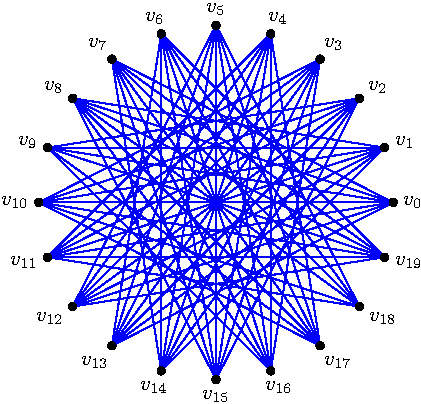
\includegraphics{example/figure} % not necessary to give extension - now you can shift between compiling to ps or to pdf without any problems
 
\caption[Do not end short caption with full-stop]{Each figure must be supplied with a long caption, making the figure stand-alone and ended with a full-stop.}

\end{figure}





\newpage





% SUBFIG EXAMPLE
%================
%
% usage: \subfloat[][caption]{...figure code...\label{label}}

The subfigures are Figures \subref{firstfigure}, \subref{secondfigure}, \subref{thirdfigure} and \subref{fourthfigure}.

\begin{figure}
\centering

\subfloat[][First subcaption (No full-stop)]{
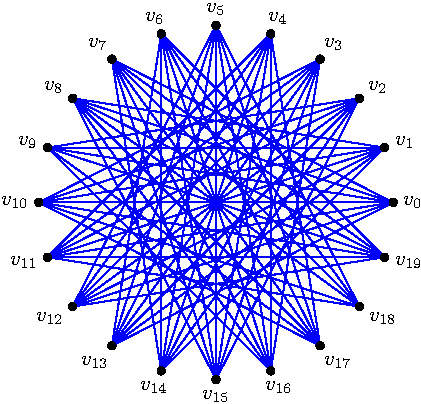
\includegraphics{example/figure}
\label{firstfigure}
}
\quad
\subfloat[][Second subcaption (No full-stop)]{
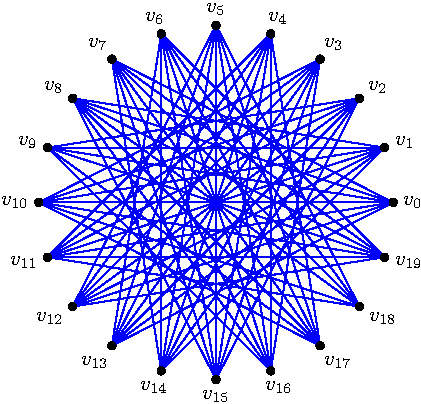
\includegraphics{example/figure}
\label{secondfigure}
}
\\
\subfloat[][Third subcaption (No full-stop)]{
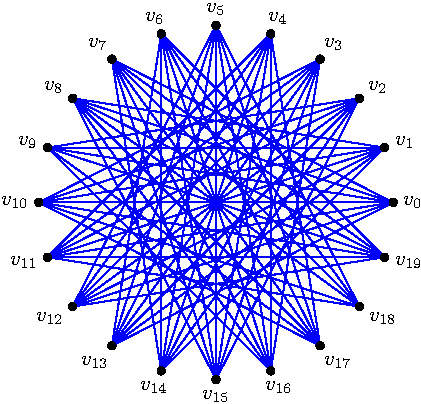
\includegraphics{example/figure}
\label{thirdfigure}
}
\quad
\subfloat[][Fourth subcaption (No full-stop)]{
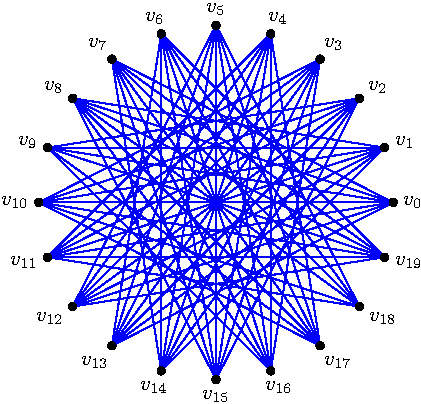
\includegraphics{example/figure}
\label{fourthfigure}
}
\caption[Do not end short caption with full-stop]{End the main caption with a full-stop, but not each of the sub-figure captions!}
\label{thislabel}
\end{figure}


\clearpage{}

\section{Deuxième section}%
\label{sec:section2}

\subsection{Exemples de code source}%
\label{sec:codessources}

\blindtext[1]
\begin{listing}[H]
\begin{pythoncode}
def get_path_leaf(path):
    """ return the leaf of a path. """
    if not isinstance(path, str):
        path = str(path)
    head, tail = ntpath.split(path)
    return tail or ntpath.basename(head)
\end{pythoncode}
\caption{SPARQL Endpoint}%
\label{lst:SPARQL Endpoint}
\end{listing}

\blindtext[2]


\begin{listing}[H]
\begin{minted}[linenos]{python}
a = 2
\end{minted}
\caption{caption}%
\label{lst:label}%
\end{listing}

\begin{listing}[H]
\pythonfile{\codefolder{hello-world.py}}
\caption{This piece of code is an included file}%
\label{lst:included-code}%
\end{listing}



\subsection{Sous section présentant les listes}

\subsubsection{Itemize}

List are really easy to create
 
\begin{itemize}
  \item One entry in the list
  \item Another entry in the list
\end{itemize}

\subsubsection{Enumerate}

\begin{enumerate}
  \item The labels consists of sequential numbers.
  \item The numbers starts at 1 with every call to the enumerate environment.
\end{enumerate}


\subsubsection{Nested Lists}

\begin{enumerate}
   \item The labels consists of sequential numbers.
   \begin{itemize}
     \item The individual entries are indicated with a black dot, a so-called bullet.
     \item The text in the entries may be of any length.
   \end{itemize}
   \item The numbers starts at 1 with every call to the enumerate environment.
\end{enumerate}




\clearpage{}

\end{document}


\documentclass[../main/main.tex]{subfiles}

\begin{document}

\onlyinsubfile{%
    % Used to color citations and references
\hypersetup{linkcolor=maincolor, citecolor=maincolor}

\iftoggle{minitocchapter}{%
    \changetocstyle{}
}{}

\thispagestyle{mainmatterstyle}
\pagestyle{mainmatterstyle}

\mainmatter{}

%
    \setcounter{chapter}{1}
}

% =====================================
% Chapitre 2
% =====================================
\chapter{Titre du deuxième chapitre un peu plus long}%
\chaptermark{Nom plus court pour le chapitre}%
\label{chap:label-chapitre-2}%
\chaptertoc{}

\section{Deuxième section}%
\label{sec:chap2section2}

\subsection{Sous-sous sections et paragraphes}%
\label{ssec:sectionandparagraphs}

\subsubsection*{Sous sous section non numérotée}

\blindtext[8]

\paragraph{Titre du paragraph} \blindtext[9]



\subsection{Sous section présentant divers choses utiles}

\paragraph{Les notes de bas de page} Voici du texte et une référence\footnote{Note de pas de page} à une note de bas de page.


\clearpage{}

\section{Section pour présenter les tableaux et références}%
\label{sec:section1-chap2}

\subsection{Sous section avec des tableaux}%
\label{sec:subsectiontableau}

\subsubsection{Tableau simple}

\begin{table}[h!]
    \centering
    \begin{tabular}{ |c|c|c| } 
        \hline
        cell1 & cell2 & cell3 \\ 
        cell4 & cell5 & cell6 \\ 
        cell7 & cell8 & cell9 \\ 
        \hline
    \end{tabular}
    \caption{Tableau simple}%
    \label{table:tableausimple}
\end{table}


\subsubsection{Tableau plus complexe}

\begin{table}[h!]
    \begin{tabular}{ |p{3cm}||p{3cm}|p{3cm}|p{3cm}|  }
        \hline
        \multicolumn{4}{|c|}{Country List} \\
        \hline
        Country Name     or Area Name& ISO ALPHA 2 Code &ISO ALPHA 3 Code&ISO numeric Code\\
        \hline
        Afghanistan   & AF    &AFG&   004\\
        Aland Islands&   AX  & ALA   &248\\
        Albania &AL & ALB&  008\\
        Algeria    &DZ & DZA&  012\\
        American Samoa&   AS  & ASM&016\\
        Andorra& AD  & AND   &020\\
        Angola& AO  & AGO&024\\
        \hline
    \end{tabular}
    \centering
    \caption{Tableau un peu plus complexe}%
    \label{table:tableaucomplexe}
\end{table}




%!TEX program = XeLaTeX
%!TeX root =main.tex

\bibliography{paper.bib}

%%% Local Variables: 
%%% mode: latex
%%% TeX-master: "main.tex"
%%% End: 


\clearpage{}

\end{document}


\input{data/chap3}
\input{data/chap4}
\input{data/chap5}
\input{data/chap6}

%==============================================================
\backmatter

% The following two commands are all you need in the
% initial runs of your .tex file to
% produce the bibliography for the citations in your paper.
{
\bibliographystyle{abbrv}
\bibliography{data/thesis}
}
% You must have a proper ".bib" file
%  and remember to run:
% latex bibtex latex latex
% to resolve all references

%==============================================================

% acknowledgement

\clearpage
\thispagestyle{plain}
\phantomsection
\addcontentsline{toc}{chapter}{Acknowledgment}

\centerline{\zihao{3}\bfseries Acknowledgment}

\linespread{1.4}\zihao{-4}
\bigskip

I would like to thank my mentor Dr.\,Xu Xiaodong for his support and patience throughout the whole writing and editing process of this thesis. My gratefulness also goes to Liu Yunhan and Zhong Yuling who helped me to solve crucial problems in experiment design and implementation.

The thesis is typeset with \LaTeX. When preparing the format template, I got much help from numerous dedicated members of different \LaTeX\ communities, to whom I express my dearest thankfulness.

\end{document}
